%-----------------------------------------------------------------%
% 2015 - 2025 Emerson Ribeiro de Mello - mello@ifsc.edu.br
% 
% 2025/04/16 versão 2
% 
% Modelo de monografia para o Instituto Federal de Santa Catarina
% 
% Adaptação do documento abnTeX2: Modelo de Trabalho Acadêmico
% para ficar de acordo com o "Manual de normalização de trabalhos
% acadêmicos do Sistema de Bibliotecas integradas do IFSC (SiBI/IFSC)  - rev 08abr25"
% disponível em  https://www.ifsc.edu.br/documentos-uteis. Acessado em 2025-04-16
%-----------------------------------------------------------------%
\documentclass[
    12pt,				% tamanho da fonte
    openright,			% capítulos começam em pág ímpar (insere página vazia caso preciso)
    oneside,			% para impressão em frente e verso, use "twoside"
    a4paper,			% tamanho do papel. 
    % -- opções da classe abntex2 --
    chapter=TITLE,		% títulos de capítulos convertidos em letras maiúsculas
    section=TITLE,		% títulos de seções convertidos em letras maiúsculas
    english,			% idioma adicional para hifenização
    brazil				% o último idioma é o principal do documento
]{ifscthesis}

% Para gerar texto de exemplo
\usepackage{lipsum} 

% Arquivo com as referências bibliográficas
\addbibresource{referencias.bib}


% Capa

%-----------------------------------------------%
% Para alterar o gênero dos comandos orientador
% e coorientador.
%-----------------------------------------------%
% \renewcommand{\orientadorname}{Orientadora:}
\renewcommand{\coorientadorname}{Coorientadora:}
%-----------------------------------------------%


%-----------------------------------------------%
% Informações de dados para CAPA e FOLHA DE ROSTO
%-----------------------------------------------%
\titulo{Modelo de Trabalho Acadêmico com \abnTeX}
\autor{Nome do Aluno}
\local{São José - SC}
\data{agosto/2022}
\orientador{Prof. Orientador da Silva, Dr.}
\coorientador{Profa. Fulana da Silva, Dra.}
\instituicao{%
  Instituto Federal de Santa Catarina -- IFSC
  \par
  Campus São José
  \par
  Engenharia de Telecomunicações}
\tipotrabalho{Monografia (Graduação)}
%-----------------------------------------------%




%-----------------------------------------------%
% O preambulo deve conter o tipo do trabalho, o objetivo, o nome da instituição e a área de concentração 
\preambulo{Monografia apresentada ao Curso de Engenharia de Telecomunicações do campus São José do Instituto Federal de Santa Catarina para a obtenção do diploma de Engenheiro de Telecomunicações.}

\textoaprovacao{Este trabalho foi julgado adequado para obtenção do título de Engenheiro de Telecomunicações, pelo Instituto Federal de Educação, Ciência e Tecnologia de Santa Catarina, e aprovado na sua forma final pela comissão avaliadora abaixo indicada.}
%-----------------------------------------------%

%-----------------------------------------------%
% Estilo de cabeçalho que só contém o número da 
% página e uma linha
%-----------------------------------------------%
\makepagestyle{cabecalholimpo}
\makeevenhead{cabecalholimpo}{\thepage}{}{} % páginas pares
\makeoddhead{cabecalholimpo}{}{}{\thepage} % páginas ímpares
% \makeheadrule{cabecalholimpo}{\textwidth}{\normalrulethickness} % linha
%-----------------------------------------------%



% Abreviaturas, siglas e símbolos
\makeglossaries
% \setabbreviationstyle[acronym]{long-postshort-user}
\setabbreviationstyle[acronym]{long-short-user}
\glssetcategoryattribute{acronym}{nohyperfirst}{true}
% \glssetcategoryattribute{acronym}{nohyper}{true}

% ------------------------------------%
%  Como usar os comandos do glossário
% ------------------------------------%
% \gls{TLS} - Na 1a. vez, texto por extenso + sigla. Nas chamadas subsequentes somente a sigla
% \glspl{IdP} - Para colocar s como prefixo da sigla
% \Gls{} - Inicial em maiúscula
% \glsxtrfull{} - texto por extenso + sigla
% \glsxtrfullpl{} - texto por extenso no plural + sigla
% \glsxtrshort{} - somente a sigla
% \glsxtrlong{} - somente o texto por extenso

%  Caso queira criar uma entrada que tenha tradução para inglês, use o parâmetro user1. 
%      Veja exemplo abaixo para Credenciais Verificáveis
% 
% Caso queira criar plural, use o parâmetro longplural. Veja exemplo para IAA
% ------------------------------------%

\newacronym
{json} % rótulo 
{JSON} % sigla
{\textit{JavaScript Object Notation}} % por extenso


\newacronym{ABNT}{ABNT}{Associação Brasileira de Normas Técnicas}

\newacronym{abnTeX}{abnTeX}{ABsurdas Normas para TeX}

\newacronym[longplural={Autoridades Certificadoras}]{AC}{AC}{Autoridade Certificadora}

\newacronym{AES}{AES}{\textit{Advanced Encryption Standard}}

\newacronym{TLS}{TLS}{\textit{Transport Layer Security}}

\newacronym{TPC}{TPC}{Terceira Parte Confiável}

\newacronym{IFSC}{IFSC}{Instituto Federal de Santa Catarina}
\glsxtrnewsymbol[description={conjunto vazio}]
{emptyset}% rótulo (será usado na ordenação na lista de símbolos)
{\ensuremath{\emptyset}}% símbolo


\glsxtrnewsymbol[description={número Pi}]
{pi}% rótulo (será usado na ordenação na lista de símbolos)
{\ensuremath{\pi}}% símbolo


\begin{document}
% Seleciona o idioma do documento (conforme pacotes do babel)
\selectlanguage{brazil}




%-----------------------------------------------%
% ELEMENTOS PRÉ-TEXTUAIS
%-----------------------------------------------%
\imprimircapa
\imprimirfolhaderosto

%-----------------------------------------------%
% Ficha catalográfica
%-----------------------------------------------%

% Pegue com a Biblioteca do IFSC um PDF com a 
% ficha correta, salve o arquivo no diretório
% deste projeto e descomente as linhas abaixo

% \begin{fichacatalografica}
%     \includepdf{ficha-catalografica.pdf}
% \end{fichacatalografica}

%-----------------------------------------------%
% folha de aprovação
%-----------------------------------------------%
\begin{folhadeaprovacao}

    \begin{center}
        {\ABNTEXchapterfont\normalfont\large\imprimirautor}

        \vspace*{2cm}

        \ABNTEXchapterfont\normalfont\large\imprimirtitulo
        
    
        \vspace*{2cm}

\hspace{.45\textwidth}
\begin{minipage}{.5\textwidth}
\SingleSpacing
{\normalsize Monografia apresentada ao Curso de Engenharia de Telecomunicações do Instituto Federal de Santa Catarina, para a obtenção do título de bacharel em Engenharia de Telecomunicações.}
\end{minipage}%
        
        \vspace*{2cm}

        % Essa data de aprovação deve ser colocada após a defesa e aprovação do trabalho
        \imprimirlocal, 16 de abril de 2025.

    \end{center}

    \vfill

    \setlength{\ABNTEXsignskip}{1.5cm}
    \assinatura{\imprimirorientador \\[.5em] Instituto Federal de Santa Catarina}     
    \assinatura{Professor Fulano, Dr. \\[.5em] Instituto Federal de Santa Catarina }
    \assinatura{Professora Fulana, Dra.  \\[.5em] Instituto Federal de Santa Catarina}
    % \assinatura{\textbf{Professor Beltrano, Dr.} \\[.5em] Instituto Z}
  
\end{folhadeaprovacao}
%-----------------------------------------------%

\begin{dedicatoria}
\vspace*{\fill}
\begin{flushright}
\begin{minipage}{0.5\textwidth}
        
    Aos meus pais, que sempre acreditaram em mim, e me ensinaram a sonhar.

\end{minipage}
\end{flushright}
\vspace*{3cm}
\end{dedicatoria}
\begin{agradecimentos}
    
    Agradeço à minha família, que sempre esteve ao meu lado, me apoiando e incentivando a seguir em frente. Vocês são a minha base e a razão pela qual busco sempre o melhor.
    
    Agradeço especialmente ao meu orientador, Professor Fulano, pela orientação e apoio durante todo o processo de elaboração deste trabalho. Sua experiência e conhecimento foram fundamentais para o meu aprendizado e crescimento acadêmico.
    
    Agradeço ao Instituto Federal de Santa Catarina, que me proporcionou uma formação sólida e de qualidade, e a todos os professores que contribuíram para o meu aprendizado.
    
    Agradeço também aos meus colegas de curso, que compartilharam comigo momentos de aprendizado e crescimento. Juntos, enfrentamos os desafios e celebramos as conquistas.
    
\end{agradecimentos}
\begin{epigrafe}
\vspace*{\fill}
\begin{flushright}
\begin{minipage}{0.5\textwidth}
%  Use o comando \cite para referenciar a citação
``Sempre que te perguntarem se podes fazer um trabalho, respondas que sim e te ponhas em seguida a aprender como se faz.'' (NOME, ANO)
\end{minipage}
\end{flushright}
\end{epigrafe}
% ajusta o espaçamento dos parágrafos do resumo
\setlength{\absparsep}{18pt} 


\begin{resumo}
    O resumo deve ressaltar o objetivo, o método, os resultados e as conclusões do documento. A ordem e a extensão destes itens dependem do tipo de resumo (informativo ou indicativo) e do tratamento que cada item recebe no documento original. Utilize frases concisas e afirmativas. Explique o tema principal do trabalho na primeira frase. Use o verbo na voz ativa e na terceira pessoa do singular. 
    
    Palavras-chave: latex. abntex. editoração de texto.
\end{resumo}



%-----------------------------------------------%
\begin{resumo}[Abstract]
\begin{otherlanguage*}{english}
    This is the english abstract.
\vspace{\onelineskip}

\noindent 
Keywords: latex. abntex. text editoration.
\end{otherlanguage*}
\end{resumo}
%-----------------------------------------------%


%-----------------------------------------------%
% LISTAS
%-----------------------------------------------%
% Lista de ilustrações
\pdfbookmark[0]{\listfigurename}{lof}
\listoffigures*
\cleardoublepage

% Lista de quadros
\pdfbookmark[0]{\listofquadrosname}{loq}
\listofquadros*
\cleardoublepage

% Lista de tabelas
\pdfbookmark[0]{\listtablename}{lot}
\listoftables*
\cleardoublepage

% Lista de códigos
\pdfbookmark[0]{\lstlistlistingname}{lol}
\begin{KeepFromToc}
\lstlistoflistings
\end{KeepFromToc}
\cleardoublepage

% Lista de abreviaturas
\printglossary[type=\acronymtype,nonumberlist,title=Lista de abreviaturas e siglas]
\cleardoublepage

% Lista de símbolos
\printglossary[type=symbols,nonumberlist,title=Lista de símbolos]
\cleardoublepage

% Sumário

\pdfbookmark[0]{\contentsname}{toc}
\tableofcontents*
\cleardoublepage

%-----------------------------------------------%
% ELEMENTOS TEXTUAIS
%-----------------------------------------------%
\pagestyle{cabecalholimpo}
\aliaspagestyle{chapter}{cabecalholimpo}


\chapter{Introdução}\label{cap:introducao}


A introdução abre o trabalho propriamente dito. Tem a finalidade de apresentar os motivos que levaram o autor a realizar a pesquisa, o problema abordado, os objetivos e a justificativa. O objetivo principal da introdução é situar o leitor no contexto da pesquisa. O leitor deverá perceber claramente o que foi analisado, como e por que, as limitações encontradas, o alcance da investigação e suas bases teóricas gerais. Ela tem, acima de tudo, um caráter didático de apresentar o que foi investigado, levando-se em conta o leitor a que se destina e a finalidade do trabalho~\cite{ifsc:manual:normalizacao}. 

Assim, na introdução contextualize o tema, delimite o assunto, apresente um rápido histórico do problema e das soluções porventura já apresentadas, com breve revisão crítica das investigações anteriores; faça referência às fontes de material, aos métodos seguidos, às teorias ou aos conceitos que embasam o desenvolvimento e a argumentação, às eventuais faltas de informação, ao instrumental utilizado. A introdução deverá conter, ainda:

\begin{itemize}
   \item Justificativa -- trata-se da relevância, o motivo pelo qual tal pesquisa deve ser realizada. Justifica-se aqui a escolha do tema, a delimitação feita e a relação que o pesquisador possui com ele. Procura-se demonstrar a legitimidade, a pertinência, o interesse e a capacidade do pesquisador em lidar com o referido tema. Deve-se fazer o mesmo em relação ao problema e à hipótese, mostrando a relevância científica do tema para o pesquisador. Deve-se fazer, então, nesta parte, a justificativa para o tema, para o problema e para a hipótese, nos termos em que foram formulados na fase de elaboração do projeto de pesquisa;
   
   \item Definição do problema -- um problema decorre de um aprofundamento do tema. Ele deve delimitar a pesquisa. Diversos autores sugerem que o problema deve ter algumas características, tais como: a) deve ser formulado como pergunta - isso facilita sua identificação por quem consulta o projeto de pesquisa; b) deve ser claro e preciso; c) deve ser delimitado a uma dimensão variável, pois muitas vezes, o problema é formulado de uma maneira muito ampla, impossível de ser investigado 
   
   \item Objetivo geral e objetivos específicos -- detalhado dentro das seções abaixo.
\end{itemize}

\section{Objetivos}

Neste item deverá ser indicado claramente o que se deseja fazer, o que se pretende alcançar. É fundamental que estes objetivos sejam possíveis de serem atingidos. Geralmente se formula um objetivo geral articulando-o a outros objetivos mais específicos.

\subsection{Objetivo geral}

Procura-se determinar\footnote{Atenção! Inicie a frase com um verbo abrangente e no infinitivo, como: compreender, saber, avaliar, verificar, constatar, analisar, desenvolver, conhecer, entender, levantar, mapear, identificar.}, com clareza e objetividade, o seu propósito com a realização da pesquisa. Deve-se estar atento ao fato de que nesta pesquisa, em nível de graduação ou pós-graduação, os propósitos são essencialmente acadêmicos, como mapear, identificar, levantar, diagnosticar, traçar o perfil ou historiar determinado assunto específico dentro de um tema. Um objetivo bem redigido explica o quê, com o quê (quem), por meio de quê, onde, quando sobre a pesquisa.

\subsection{Objetivos específicos}

Significa aprofundar as intenções expressas no objetivo geral. Propõe-se mapear, identificar, levantar, diagnosticar, traçar o perfil ou historiar determinado assunto específico dentro de um tema. Assim, para elaborar os objetivos específicos deve-se:

\begin{itemize}
   \item detalhar o objetivo geral mostrando o que se pretende alcançar com a pesquisa;
   \item tornar operacional o objetivo geral, indicando exatamente o que será realizado na pesquisa;
   \item usar verbos que admitam poucas interpretações e no infinitivo, como: identificar, caracterizar, comparar, testar, aplicar, observar, medir, localizar, selecionar, distinguir.
\end{itemize}


% \section{Organização do texto}

% O texto está organizado da seguinte forma: No \autoref{cap:revisao} é apresentado um pouco mais de como fazer um outro capítulo, apresentando ainda formas para inserir figuras. No \autoref{cap:proposta} é apresentado uma forma para adicionar uma tabela. Por fim, no \autoref{cap:conclusoes} são apresentadas as conclusões sobre este trabalho.
\chapter{Revisão bibliográfica}\label{cap:revisao}

É uma análise comentada sobre o que já foi publicado sobre o assunto da pesquisa, buscando mostrar os pontos de vista convergentes e divergentes entre os autores. Traça-se um quadro teórico e elabora-se a estruturação conceitual que subsidiará o desenvolvimento da pesquisa. A revisão de literatura permitirá um mapeamento de quem já escreveu e o que já foi escrito sobre o assunto ou o problema de pesquisa.


\section{Quadros}\label{sec:quadros}


Um quadro é formado por linhas horizontais e verticais, sendo fechado em todas as suas extremidades e, geralmente, é utilizado para expressar dados qualitativos. Verifique um exemplo de utilização no \autoref{quadro:exemplo}.


\begin{quadro}[htb]
\caption{Exemplo de quadro}\label{quadro:exemplo}
\begin{tabular}{|l|r|r|r|}
    \hline
    \textbf{Pessoa} & \textbf{Idade} & \textbf{Peso} & \textbf{Altura} \\ \hline
    Marcos & 26    & 68   & 178    \\ \hline
    Ivone  & 22    & 57   & 162    \\ \hline
    ...    & ...   & ...  & ...    \\ \hline
    Sueli  & 40    & 65   & 153    \\ \hline
\end{tabular}
\fonteproprioautor
\end{quadro}

No \autoref{quadro:docentes} são listados os docentes do curso.

\begin{quadro}[htb]
    \centering
    \caption{Listagem dos docentes do curso}\label{quadro:docentes}
    \footnotesize
    \begin{tabular}{|l|l|l|}
    \hline
    \textbf{Docente} & \textbf{Formação acadêmica}    & \textbf{UCs}                               \\ \hline
    Fulano de tal    & Engenharia de Telecomunicações & Antenas, Radiotransmissão, Circuitos de RF \\ \hline
    Nononono         & Ciências da Computação         & Programação, Sistemas Distribuídos         \\ \hline
    Sicrano          & Engenharia Elétrica            & Análise de Circuitos, Sinais e Sistemas    \\ \hline
    \end{tabular}
    \fonteproprioautor
\end{quadro}


\section{Tabelas}\label{sec:tabelas}

De acordo com \textcite{ibge1993}, tabelas são ilustrações com dados estatísticos numéricos. A moldura de uma tabela não deve ter traços verticais que a delimitem à esquerda e à direita. Quando houver necessidade de se destacar parte do cabeçalho ou parte dos dados numéricos estes devem ser estruturados com um ou mais traços verticais paralelos adicionais. Linhas horizontais só se admitem no cabeçalho e no rodapé. 

Tabelas não devem figurar dados em branco. Assim, em um tabela:

\begin{itemize}
    \item Traço indica dado inexistente;
    \item Reticências indicam dado desconhecido;
    \item Zero deve ser usado quando o dado for menor que a metade da unidade adotada para a expressão do dado.
\end{itemize}

As tabelas devem ser citadas no texto, inseridas o mais próximo possível do trecho a que se referem e padronizadas segundo as Normas de Apresentação Tabular do IBGE. Os números sempre devem ser alinhados à direita, veja um exemplo na \autoref{tab:publicacoes}.

\begin{table}[htb]
    \ABNTEXfontereduzida
    \centering
    \caption{Produção dos docentes do curso}
    \label{tab:publicacoes}
    \begin{tabular}{p{3.3cm} r r R{2cm}}\toprule
        Produto científico & \multicolumn{2}{c}{Período} &  \\ \cmidrule{2-3}
                   & 2000-2010 & 2010-2020 & Total \\ \midrule
        Artigo nacional & 10 & 20 & 30 \\ 
        Artigo internacional & 5 & 5 & 10 \\
        Orientações de TCC & 30 & 40 & 70 \\ \midrule 
        Total & 45 & 65 & 110 \\

        \bottomrule
    \end{tabular}

    % Comando para adicionar a fonte de elaboração do autor
    \fonteproprioautor

\end{table}



\section{Figuras}\label{sec:figuras}

As figuras são bastante úteis para ajudar expressar o funcionamento, modelo, etc. de alguma parte de seu trabalho. O \textit{Inkscape}\footnote{\url{https://inkscape.org/pt-br}.} é um \textit{software} livre para criação de desenhos vetoriais e que permite exportar os desenhos para os formatos PDF, PNG etc. O \textit{site} \url{https://diagrams.net} também uma boa opção para criar figuras.

A inclusão de figuras no texto necessita que algumas regras sejam atendidas. São essas:

\begin{itemize}
	\item As figuras deverão ser de alta qualidade;
	\begin{itemize}
		\item Evite colocar fotos e outras figuras complexas;
		\item Opte por figuras simples e que realmente expressem algo, mesmo quando impressas em preto e branco;
	\end{itemize}
	\item Em \LaTeX~as figuras deverão estar nos formatos: \texttt{PDF}, \texttt{JPG} ou \texttt{PNG};
	\item Toda figura deverá possuir uma legenda;
	\item Toda figura deverá ser referenciada em alguma parte do texto.
\end{itemize}

A \autoref{fig:escrita} foi inserida no texto para mostrar como fazer tal inserção em \LaTeX. Vale lembrar que toda figura inserida deverá ser, em algum momento, referenciada no texto. 

\begin{figure}[ht]
	\centering
	\caption{Uma pessoa escrevendo sua monografia}\label{fig:escrita}
	
\includegraphics[width=5cm]{figuras/man}
    \fonte{\textcite{openclipart}}
\end{figure}


\subsection{Mascotes}\label{sec:mascotes}


A \autoref{fig:mascotes} ilustra uma forma de incluir duas figuras, lado a lado, usando o pacote \texttt{subcaption}. A \autoref{fig:mascote1} ilustra o mascote do \LaTeX~estudando. Já na \autoref{fig:mascote2} o mascote aparece apresentando algum assunto. 

\begin{figure}[ht]
	\centering
	\caption{O mascote do~\LaTeX~em diferentes poses}\label{fig:mascotes}

	\begin{subfigure}[t]{.4\textwidth}
        \centering
        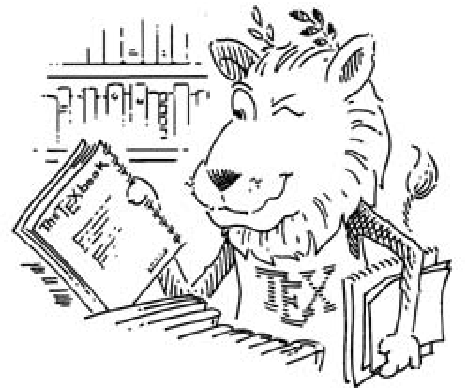
\includegraphics[width=\textwidth]{figuras/lion.pdf}
        \caption{O mascote estudando}\label{fig:mascote1}
    \end{subfigure}
    \begin{subfigure}[t]{.4\textwidth}
        \centering
        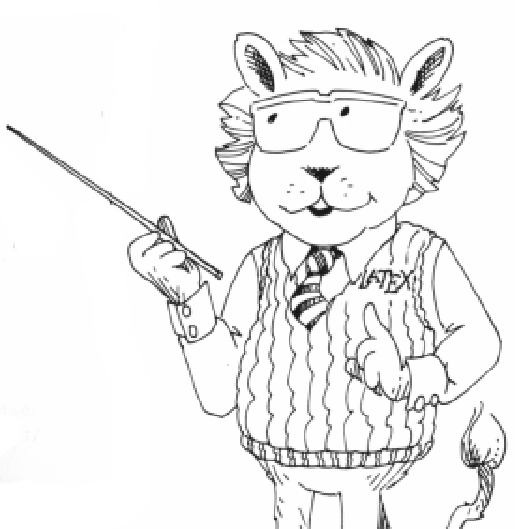
\includegraphics[width=\textwidth]{figuras/latex_lion.pdf}
        \caption{O mascote ensinando}\label{fig:mascote2}
    \end{subfigure}
\end{figure}

\chapter{Proposta}\label{cap:proposta}


\section{Incluindo trechos de códigos}\label{sec:codigos}

Em alguns casos é desejado incluir trechos de códigos no documento. O \LaTeX~oferece inúmeras maneiras para isto e o pacote \textbf{listings} é conhecido por apresentar um dos melhores resultados. A \autoref{cod:olamundo} apresenta o código em \textit{shell script} para o complexo problema do ``Olá mundo!''. A \autoref{cod:matlab} apresenta um trecho de código em MatLab e por fim, na \autoref{cod:pessoa} é ilustrado um aluno representado em um documento JSON.

\lstinputlisting[language=csh,caption={Olá mundo em shell script},label=cod:olamundo]{codigos/ola.sh}

\lstinputlisting[language=matlab,caption={Um pequeno código em MatLab},label=cod:matlab]{codigos/matlab.m}

\lstinputlisting[language=json,caption={Aluno representado em JSON},label=cod:pessoa]{codigos/pessoa.json}


\section{Como apresentar equações}\label{sec:equacoes}

O \LaTeX é um pacote feito para a preparação de textos impressos de alta qualidade, especialmente
para textos matemáticos. Ele foi desenvolvido por Leslie Lamport a partir do programa~\TeX~criado por Donald Knuth.

Fórmulas matemáticas são produzidas diretamente no arquivo fonte texto. Isto significa que o~\LaTeX~deve ser informado que o texto que vem a seguir é uma fórmula e também quando ela termina e o texto normal recomeça. As fórmulas podem ocorrer em uma linha de texto como $ ax^2 + bx + c = 0 $, ou destacada do texto principal como os exemplos apresentados na \autoref{e_c2_eq1} e \autoref{e_c2_eq2}.

\begin{equation}
 x=\frac{-b\pm\sqrt{b^2-4ac}}{2a}
\label{e_c2_eq1}
\end{equation}

\begin{align}
f(x) &= x^2 \nonumber\\
g(x) &= \dfrac{1}{\sqrt{x}} \nonumber\\
F(x) &= \int^a_b \frac{1}{3}x^3
\label{e_c2_eq2}
\end{align}


\section{Usando siglas, abreviaturas e símbolos}

Algumas vezes nos deparamos com textos cheios de siglas ou símbolos. Existem diversos pacotes e formas para gerar glossário, lista de acrônimos, lista de símbolos etc. com \LaTeX. Neste parágrafo é feito uso de comandos definidos no pacote \textit{glossaries-extra}\footnote{\url{https://www.ctan.org/pkg/glossaries-extra}}. A listagem de acrônimos fica dentro do arquivo \texttt{pretextuais/abreviacoes-siglas.tex} e a listagem de símbolos fica dentro do arquivo \texttt{pretextuais/simbolos.tex}.

O símbolo \gls{emptyset} representa um conjunto vazio, já o símbolo \gls{pi} representa o número Pi. O protocolo \gls{TLS} deve ser empregado sempre que se deseja garantir a integridade e a confidencialidade das mensagens trocadas pela rede. O \gls{TLS} é hoje utilizado por diversas aplicações. Como faz tempo que eu não falo do \glsxtrfull{TLS} eu chamo o nome completo mais a sigla, ajudando o meu leitor a lembrar da sigla \glsxtrshort{TLS}. Existem as \glsxtrfullpl{AC} que são bem importante. Este documento segue as normas da \gls{ABNT} e para isso faz uso do pacote \gls{abnTeX}.

Abaixo são apresentados os comandos providos pelo pacote \textit{glossaries-extra}:

\begin{itemize}
    \item \verb+\gls{rotulo}+ -- Na primeira vez que o acrônimo for chamado será impresso o valor por extenso e o acrônimo. Ex: \verb+\gls{IFSC}+ irá imprimir Instituto Federal de Santa Catarina (IFSC). Nas demais vezes irá imprimir somente o acrônimo;
    \item \verb+\glspl{rotulo}+ -- Semelhante ao anterior, mas imprime a forma no plural;
    \item \verb+\glsxtrshort{rotulo}+ -- Para imprimir somente o acrônimo;
    \item \verb+\glsxtrlong{rotulo}+ -- Para imprimir somente o valor por extenso;
    \item \verb+\glsxtrfull{rotulo}+ -- Para imprimir o valor por extenso e o acrônimo, mesmo que o acrônimo já tenha sido invocado previamente.
\end{itemize}



\section{Referências bibliográficas}\label{sec:referencias}

A formatação das referências bibliográficas conforme as regras da ABNT são um dos principais objetivos do \abnTeX. Consulte os manuais \textcite{abntex2cite} e \textcite{abntex2cite-alf} para obter informações sobre como utilizar as referências bibliográficas.


O uso de citações ao londo do texto é uma prática desejável. Por exemplo, em \cite{lamport94} é apresentado um documento sobre a preparação de textos usando \LaTeX. Já em \cite{goossens94} é apresentada uma lista de referências rápidas para realizar as mais simples tarefas em \LaTeX.

É o caso em que você menciona \emph{explicitamente} o autor da referência na sentença, algo
do tipo ``Fulano (1900)''. Neste caso o nome do autor é escrito
normalmente. Para isso use o comando \verb+\textcite+.

A ironia será assim uma \ldots\ proposta  por \textcite{lamport94}. Em \cite{exemplo} foi usado para ilustrar como uma \textit{URL} deve aparecer na seção das referências. Este documento segue as normas da ABNT e para isso faz uso do pacote abnTeX.


% ---
\section{Citações diretas}
\label{sec-citacao}
% ---

\index{citações!diretas}Utilize o ambiente \texttt{citacao} para incluir
citações diretas com mais de três linhas:

\begin{citacao}
As citações diretas, no texto, com mais de três linhas, devem ser
destacadas com recuo de 4 cm da margem esquerda, com letra menor que a do texto
utilizado e sem as aspas. No caso de documentos datilografados, deve-se
observar apenas o recuo \cite[5.3]{NBR10520:2002}.
\end{citacao}

Use o ambiente assim:

\begin{verbatim}
\begin{citacao}
As citações diretas, no texto, com mais de três linhas [\ldots] 
deve-se observar apenas o recuo \cite[5.3]{NBR10520:2002}.
\end{citacao}
\end{verbatim}

O ambiente \texttt{citacao} pode receber como parâmetro opcional um nome de
idioma previamente carregado nas opções da classe. Nesse
caso, o texto da citação é automaticamente escrito em itálico e a hifenização é
ajustada para o idioma selecionado na opção do ambiente. Por exemplo:

\begin{verbatim}
\begin{citacao}[english]
Text in English language in italic with correct hyphenation.
\end{citacao}
\end{verbatim}

Tem como resultado:

\begin{citacao}[english]
Text in English language in italic with correct hyphenation.
\end{citacao}

\index{citações!simples}Citações simples, com até três linhas, devem ser
incluídas com aspas. Observe que em \LaTeX as aspas iniciais são diferentes das
finais: ``Amor é fogo que arde sem se ver''.


\chapter{Conclusões}\label{cap:conclusoes}

Este trabalho procurou mostrar como deverá ser a apresentação da monografia a ser submetida à Coordenação do Curso de Engenharia de Telecomunicações do IFSC para a obtenção do diploma de Bacharel em Engenharia de Telecomunicações.

No \autoref{cap:introducao} foi feita uma pequena introdução. No \autoref{cap:revisao} foi apresentado o uso de alguns ambientes flutuantes no~\LaTeX~. E no \autoref{cap:proposta} foi apresentado sobre equações e como inserir trechos de código.

Como trabalho futuro, fica a reescrita do texto deste documento de forma que ele possam indicar informações específicas a formatação do documento. Como o tamanho da fonte utilizada, o espaçamento da borda, o alinhamento e numeração das seções e capítulos etc.



% Imprimir Referências
\printbibliography[title={Referências}]%

%-----------------------------------------------%
% Apêndices
%-----------------------------------------------%
\begin{apendicesenv}


\chapter{Meu primeiro apêndice}

Texto ou documento, elaborado pelo autor, a fim de complementar sua argumentação, sem prejuízo da unidade nuclear do trabalho. Os apêndices são identificados por letras maiúsculas ordenadas alfabeticamente, travessão e pelo respectivo título. 

\end{apendicesenv}

% Anexos
%-----------------------------------------------%
% Anexos
%-----------------------------------------------%
\begin{anexosenv}


\chapter{Meu primeiro assunto de anexo}

Texto ou documento não elaborado pelo autor, que serve de fundamentação, comprovação e ilustração. Os anexos são identificados por letras maiúsculas ordenadas alfabeticamente, travessões e pelos respectivos títulos. 

\chapter{Segundo assunto que pesquisei}
\lipsum[1-3]

\end{anexosenv}


\end{document}